\documentclass[12pt]{article}
\usepackage{tikz}
\usepackage{blindtext}
\usepackage{multicol}
\setlength{\columnsep}{1cm}
\title{Second multicols Demo}
\usetikzlibrary{calc}
\usepackage{graphicx}
\graphicspath{{images/}}
\usepackage[left=25mm,right=25mm,top=25mm,bottom=25mm,paper=a4paper]{geometry}
\usepackage{graphicx}
\graphicspath{{images/}}

\begin{document}

 \begin{center}
 \large \textbf {A Report on}\\[2mm]
 \LARGE \textbf {"Fake Currency Detetctor"}\\[7mm]
 
 \textbf{Submitted by :}\\[2mm]
 \end{center}
 
 
 \begin{tabular}{ c c c } 
 \textbf{Mr.Atharv Miind Davale} & \hspace{1.1in} & \textbf{ PRN :  2020032500183191} \\ [1mm] 
 \textbf {Mr.Rushikesh Rajesh Waghule} & \hspace{1.1in} & \textbf{PRN :2020032500186525}\\[1mm]
 \textbf{ Mr.Digvijay Sambhaji Shinde } & \hspace{1.1in}  & \textbf{PRN : :2020032500185166}\\[7mm]
 \end{tabular} 
 
 
 
 \begin{center}
 \large \textbf {UNDER THE GUIDANCE OF }\\[2mm]
 \large \textbf {Mr.A.M.Dyade}\\[7mm]
 \textbf {in partial fulfilment for the award of the degree} \\[2mm] of \\[2mm]
 
 \large \textbf {BACHELOR OF TECHNOLOGY}\\[2mm]
 \textbf {IN}\\[2mm]
 \textbf {DEPARTMENT OF COMPUTER SCIENCE AND ENGINEERING}\\
 \textbf {at}
 \end{center}
 
 \begin{figure}[h]
 \centering
 \includegraphics[scale=1]{sveri2logo}
\end{figure} 

\begin{center}
\textbf{SHRI VITHAL EDUCATION AND RESEARCH INSTITUTESs,\\[2mm]
College of Engineering, Pandharpur\\[3mm]
Affiliated to Punyashlok Ahilyadevi Holkar Solapur University, Solapur\\[2mm]
2023-2024}
\end{center}  
 
 \begin{tikzpicture}
[remember picture,overlay]\draw[line width = 1pt]($(current page.north west)+(0.5 in,-0.5in)$) rectangle ($(current page.south east)+(-0.5 in,1 in)$);
\end{tikzpicture} 
\clearpage


\begin{figure}[h]
 \centering
 \includegraphics[scale=1]{sveri2logo}
\end{figure}

\begin{center}
 \large \textbf { SVERI's COLLEGE OF ENGINEERING , PANDHARPUR }\\[7mm]
 \textbf{CERTIFICATE}\\[7mm]
 \end{center} 
 This is to certify that the project report entitled "Fake Currency Detector"\\[2mm] is submitted for partial fulfillment of Bachelor Degree in Computer Science And Engi\\[2mm]neering as per requirement of Punyashlok Ahilyadevi Holkar Solapur University, Solapur\\[2mm] for the academic year 2023-2024.\\[30mm] 
 

 
 \begin{tabular}{ c c c } 
 \textbf{( Mr.A.M.DYADE)} & \hspace{2.0in} & \textbf{( Mr.P.D.MANE )} \\ [1mm] 
 \textbf {Project Guide} & \hspace{2.0in} & \textbf{Project Coordinator}\\[30mm]
 \textbf{( Dr.S.P.PAWAR )} & \hspace{2.0in}  & \textbf{Dr.B.P.RONGE}\\[1mm]
 \textbf{(HOD , CSE )} & \hspace{2.0in}  & \textbf{ PRINCIPAL }\\[30mm]
 \end{tabular}
 
 \begin{center}
 \large \textbf { EXTERNAL EXAMINAR }
 \end{center} 


\begin{tikzpicture}
[remember picture,overlay]\draw[line width = 1pt]($(current page.north west)+(0.5 in,-0.5in)$) rectangle ($(current page.south east)+(-0.5 in,1 in)$);
\end{tikzpicture} 
\clearpage




\begin{center}
 \Large \textbf {Acknowledgement}\\[30mm]
 \end{center}\par
 We are pleased to acknowledge \textbf{Dr.S.P.PAWAR} ( HOD CSE ) for her valuable \\[1mm]
 guidance during the course of this project work . We extend our sincere thanks to \\[1mm]
 \textbf{Dr.P.D.MANE} who continously helped us throughout the project and without his\\[1mm]
  guidence , this project would have been an uphill task\\[5mm]\par
We are also grateful to other members of the CSE faculty members and technical staff\\[1mm]
 who cooperated with us regarding some issues\\[5mm]\par 
Last but not the least , Ms.T.A.Dhumal supervisor of Project Lab and Mr.P.D.Mane\\[1mm]
 supervisor of Database Lab as the case may be for project sessions , also cooperated with\\[1mm]
  us nicely for the smooth development of thid project . I would also like to thank my\\[1mm]
   parents and friends who helped me a lot in executing this project within the limited time\\[1mm]
    frame . \\[40mm]
   
\begin{tabular}{ c c c } 
  \hspace{3.4in} & \large \textbf{Signature : } \\ [5mm] 
 \end{tabular}      
    
   
 \begin{tabular}{ c c c c } 
  \hspace{1.1in}&\textbf{Mr.Atharv Milind Davale} & \hspace{0.5in}  & \textbf{ Sign :....................)} \\ [1mm] 
  \hspace{1.1in} &\textbf {Mr.Rushikesh Rajesh Waghule}& \hspace{0.5in}   & \textbf{Sign :.....................) }\\[1mm]
  \hspace{1.1in}  &\textbf{ Mr.Digvijay Sambhaji shinde } & \hspace{0.5in}  & \textbf{Sign :.....................) }\\[7mm]
 \end{tabular}   


\begin{tikzpicture}
[remember picture,overlay]\draw[line width = 1pt]($(current page.north west)+(0.5 in,-0.5in)$) rectangle ($(current page.south east)+(-0.5 in,1 in)$);
\end{tikzpicture} 
\clearpage


\begin{center}
 \Large \textbf {TABLE OF CONTENTS }\\[15mm]
 \end{center}


\begin{tabular}{ c c c c } 
  \textbf{Title Page} & \hspace{3.5in}  & \textbf{i} \\ [5mm] 
  \textbf{Certificate} & \hspace{3.5in}  & \textbf{ii} \\ [5mm]
  \textbf{Acknowledgement} & \hspace{2.5in}  & \textbf{iii} \\ [5mm] 
  \textbf{Synopsis} & \hspace{2.5in}  & \textbf{iv} \\ [5mm] 
  \textbf{Table of contents} & \hspace{2.5in}  & \textbf{vi} \\ [5mm] 
  \textbf{Abbreviations} & \hspace{2.5in}  & \textbf{vii} \\ [5mm] 
  \textbf{List of Figures} & \hspace{2.5in}  & \textbf{ix} \\ [5mm]  
 \end{tabular}  

\begin{tikzpicture}
[remember picture,overlay]\draw[line width = 1pt]($(current page.north west)+(0.5 in,-0.5in)$) rectangle ($(current page.south east)+(-0.5 in,1 in)$);
\end{tikzpicture} 
\clearpage

\tableofcontents

\begin{tikzpicture}
[remember picture,overlay]\draw[line width = 1pt]($(current page.north west)+(0.5 in,-0.5in)$) rectangle ($(current page.south east)+(-0.5 in,1 in)$);
\end{tikzpicture} 
\clearpage

\textbf{Abbreviation}\\[100mm]


\Large \textbf{List Of Figures}

\begin{tikzpicture}
[remember picture,overlay]\draw[line width = 1pt]($(current page.north west)+(0.5 in,-0.5in)$) rectangle ($(current page.south east)+(-0.5 in,1 in)$);
\end{tikzpicture} 
\clearpage




\begin{center}
 \LARGE \textbf {Chapter 1 }\\[10mm]
 \Large \textbf{INTRODUCTION}\\[10mm]
 \end{center}
 \section{Introduction}
\subsection{Introduction}
In the contemporary global economy, the circulation of counterfeit currency has emerged as a critical challenge, posing severe threats to financial systems, businesses, and individuals alike. The proliferation of sophisticated printing technologies and the ease of access to advanced graphic design tools have exacerbated the prevalence of fake currency, leading to substantial economic losses and eroding public trust in monetary transactions.\\[1mm]\\[1mm]
The "Fake Currency Detector" project is conceived as a proactive response to combat the rising tide of counterfeit currency. By leveraging cutting-edge technologies and innovative design principles, this project aims to develop a robust and efficient system capable of detecting fake currency in real-time. Through the implementation of advanced security features, the project seeks to establish a formidable defense against the proliferation of counterfeit money in various sectors.\\[1mm]
 
 \subsection{Need of work}
The urgency of addressing the counterfeit currency issue cannot be overstated. Counterfeit money not only poses a direct threat to financial institutions but also undermines the integrity of transactions in everyday commerce. The need for a reliable and efficient fake currency detection system is evident, considering the potential economic losses, damage to businesses, and the erosion of public confidence in monetary instruments.\\[1mm]
 \subsection{Objectives}
The primary objectives of the Fake Currency Detector project include:

\textbf{Real-Time Detection:}Develop a system capable of identifying counterfeit currency in real-time, minimizing the risk of fraudulent transactions.

\textbf{Enhanced Security Features:}l Implement advanced security measures to make currency designs more resilient against counterfeiting attempts.

\textbf{Economic Safeguarding:} Contribute to the reduction of economic losses attributed to counterfeit currency circulation.\\[1mm]

\begin{tikzpicture}
[remember picture,overlay]\draw[line width = 1pt]($(current page.north west)+(0.5 in,-0.5in)$) rectangle ($(current page.south east)+(-0.5 in,1 in)$);
\end{tikzpicture} 
\clearpage

\begin{center}
 \LARGE \textbf {Chapter 2 }\\[10mm]
 \Large \textbf{LITERATURE SURVEY}\\[10mm]
 \end{center}
 \section{LITERATURE SURVEY}
 \subsection{Existng System}
The existing systems for counterfeit currency detection predominantly rely on traditional security features such as watermarks, holograms, and special inks. While these methods have been effective to some extent, they often fall short in detecting highly sophisticated counterfeit notes produced with advanced printing technologies. The need for a more technologically advanced and robust system is apparent, prompting the development of innovative solutions.
\\[0.5mm]\textbf{Example : UV light Examination} 
: it is a relatively inexpensive method. UV light sources are widely available and affordable, making it a cost-effective solution for businesses and individuals.
\\[0.5mm]Lack of Real-Time Analysis: UV light examination does not provide real-time analysis of currency features. It requires manual inspection, which can be time-consuming and may not be suitable for high-speed transactions.
 \subsection{Problem Definition}
The main challenges in the existing counterfeit currency detection systems include a lack of adaptability to evolving counterfeiting techniques, low accuracy rates, and the inability to detect subtle anomalies in currency features. These shortcomings highlight the necessity for an updated and more intelligent system that can keep pace with the increasingly sophisticated methods employed by counterfeiters.
 \subsection{Proposed System}
The proposed Fake Currency Detector employs a combination of image processing algorithms and machine learning techniques. This allows for real-time analysis of currency features, including intricate patterns and security elements, enabling the system to identify even the most sophisticated counterfeit notes. The integration of advanced technologies aims to significantly improve the overall effectiveness of counterfeit currency detection.
 \subsection{Advantages of Proposed System}
The advantages of the proposed system include enhanced accuracy in counterfeit detection, adaptability to emerging counterfeiting techniques, and a reduction in false positives. The integration of machine learning ensures continuous learning and improvement, making the system more resilient against evolving counterfeit strategies. Moreover, the real-time processing capability enhances the efficiency of currency verification, making it a valuable asset for various industries.



\begin{tikzpicture}
[remember picture,overlay]\draw[line width = 1pt]($(current page.north west)+(0.5 in,-0.5in)$) rectangle ($(current page.south east)+(-0.5 in,1 in)$);
\end{tikzpicture} 
\clearpage





\begin{center}
 \LARGE \textbf {Chapter 3 }\\[10mm]
 \Large \textbf{SYSTEM ANALYSIS AND DESIGN}\\[10mm]
 \end{center}
 \section{System Analysis And Design}
 \subsection{Requirement Specification }
\textbf{Real-Time Currency Analysis:} The system should be capable of analyzing currency features in real-time to facilitate quick and efficient detection.

\textbf{Machine Learning Integration:} Implement machine learning algorithms to enable continuous learning and adaptation to evolving counterfeit techniques.

\textbf{User Interface:} Develop an intuitive user interface for ease of use by operators, providing clear indications of counterfeit detection results.
 \subsection{Design and Test Steps / Criteria}
1. System Architecture:\\[0.5mm]
Develop an image processing module for real-time currency analysis.\\[0.5mm]
Integrate machine learning algorithms for continuous improvement in counterfeit detection.\\[0.5mm]

2. Data Flow:\\[0.5mm]
Input: Currency images are processed using image processing and machine learning.\\[0.5mm]
Processing: The system analyzes currency features.\\[0.5mm]
Output: Real-time feedback on currency authenticity is provided.\\[0.5mm]

3. User Interface:\\[0.5mm]
Design an intuitive interface with clear indicators for counterfeit detection.\\[0.5mm]
Implement an alert system for prompt notification of suspected counterfeit notes.\\[0.5mm]

Test Steps/Criteria:\\[0.5mm]

Functional Testing:
Verify real-time analysis capability within 1 second.\\[0.5mm]
Test machine learning accuracy with a minimum 95 percent detection rate.\\[0.5mm]

Non-Functional Testing:\\[0.5mm]
Evaluate scalability with at least three currency types.\\[0.5mm]
Assess security measures to prevent unauthorized access and tampering.\\[0.5mm]
Collect usability feedback, ensuring easy operation for operators.\\[0.5mm]

\begin{tikzpicture}
[remember picture,overlay]\draw[line width = 1pt]($(current page.north west)+(0.5 in,-0.5in)$) rectangle ($(current page.south east)+(-0.5 in,1 in)$);
\end{tikzpicture} 
\clearpage

\begin{center}
 \LARGE \textbf {Chapter 4 }\\[10mm]
 \Large \textbf{METHODOLOGY / TECHNIQUES USED}\\[10mm]
 \end{center}
 \section{Methodology / Techniques Used}
 \subsection{ Image Processing and Analysis}
Methodology:\\[0.3mm]
Capture currency images.\\[0.3mm]
Preprocess images for quality.\\[0.3mm]
Extract features and recognize patterns.\\[0.3mm]

Techniques Used:\\[0.3mm]
Histogram Equalization\\[0.3mm]
Edge Detection\\[0.3mm]
Template Matching\\[0.3mm]

\subsection{Machine Learning Integration}
Methodology:\\[0.3mm]
Collect diverse dataset.\\[0.3mm]
Train models for pattern recognition.\\[0.3mm]
Enable continuous learning.\\[0.3mm]

Techniques Used:\\[0.3mm]
Supervised Learning\\[0.3mm]
Neural Networks\\[0.3mm]

\subsection{Real-Time Processing}
Methodology:\\[0.3mm]
Optimize algorithms for real-time.\\[0.3mm]
Implement parallel processing.\\[0.3mm]

Techniques Used:\\[0.3mm]
Multithreading\\[0.3mm]
GPU Acceleration\\[0.3mm]

\subsection{ Usability and Interface Design}
Methodology:\\[0.3mm]
Gather user feedback.\\[0.3mm]
Iterative design based on feedback.\\[0.3mm]

Techniques Used:\\[0.3mm]
User-Centered Design\\[0.3mm]
Prototyping\\[0.3mm]

\subsection{Testing and Validation}
Methodology:\\[0.3mm]
Functional testing for real-time analysis.\\[0.3mm]
Usability testing for interface.\\[0.3mm]
Scalability and security testing.\\[0.3mm]

Techniques Used:\\[0.3mm]
Unit Testing\\[0.3mm]
User Testing\\[0.3mm]
Penetration Testing\\[0.3mm]
 
% \begin{figure}[h]
% \centering
% \includegraphics[scale=1]{Quantum}
%  \caption{Code page -1 }
% \end{figure}
 
% \begin{tikzpicture}
%[remember picture,overlay]\draw[line width = 1pt]($(current page.north west)+(0.5 in,-0.5in)$) rectangle ($(current page.south east)+(-0.5 in,1 in)$);
%\end{tikzpicture} 
%\clearpage
 
% \begin{figure}[h]
% \centering
% \includegraphics[scale=1]{Quantum}
%  \caption{Code page -2}
% \end{figure}
 
% \begin{figure}[h]
% \centering
% \includegraphics[scale=1]{Quantum}
%  \caption{Code page -3}
% \end{figure}
 
% \begin{tikzpicture}
%[remember picture,overlay]\draw[line width = 1pt]($(current page.north west)+(0.5 in,-0.5in)$) rectangle ($(current page.south east)+(-0.5 in,1 in)$);
%\end{tikzpicture} 
%\clearpage
 
% \begin{figure}[h]
% \centering
% \includegraphics[scale=1]{Quantum}
%  \caption{Code page -4}
% \end{figure}
 
% \begin{figure}[h]
% \centering
% \includegraphics[scale=1]{Quantum}
%  \caption{Code page -5}
% \end{figure}
 
% \begin{tikzpicture}
%[remember picture,overlay]\draw[line width = 1pt]($(current page.north west)+(0.5 in,-0.5in)$) rectangle ($(current page.south east)+(-0.5 in,1 in)$);
%\end{tikzpicture} 
%\clearpage
 
% \begin{figure}[h]
% \centering
% \includegraphics[scale=1]{Quantum}
%  \caption{Code page -6}
% \end{figure}

%\begin{tikzpicture}
%[remember picture,overlay]\draw[line width = 1pt]($(current page.north west)+(0.5 in,-0.5in)$) rectangle ($(current page.south east)+(-0.5 in,1 in)$);
%\end{tikzpicture} 
%\clearpage



%\begin{center}
% \LARGE \textbf {Chapter 5 }\\[10mm]
% \Large \textbf{EXPERIMENTAL RESULTS / OUTPUTS }\\[10mm]
% \end{center}
 
% \begin{figure}[h]
% \centering
% \includegraphics[scale=1]{Quantum}
% \caption{Logo Of Application}
% \end{figure}

 
% \begin{figure}[h]
% \centering
% \includegraphics[scale=1]{Quantum}
% \caption{Login Page}
% \end{figure}
 
% \begin{figure}[h]
% \centering
% \includegraphics[scale=1]{Quantum}
%  \caption{Home Page}
% \end{figure}
% 
%\begin{tikzpicture}
%[remember picture,overlay]\draw[line width = 1pt]($(current page.north west)+(0.5 in,-0.5in)$) rectangle ($(current page.south east)+(-0.5 in,1 in)$);
%\end{tikzpicture} 
%\clearpage


\begin{center}
 \LARGE \textbf {Chapter 6 }\\[10mm]
 \Large \textbf{CONCLUSION AND FUTURE SCOPE }\\[10mm]
 \end{center}
 \large \textbf{CONCLUSION :}\\[3mm]\par

In concluding the Fake Currency Detector project, we affirm the significance of our efforts in addressing the growing challenges posed by counterfeit currency. The methodologies employed, including image processing and machine learning integration, have been instrumental in designing a system capable of real-time counterfeit detection.\\[2mm]

 \large \textbf{FUTURE SCOPE :}\\[3mm]\par
The following improvements can be made to the system ,
\begin{itemize}
\item International Currency Support:
Expand the system's capabilities to encompass a broader range of international currencies, addressing the global nature of counterfeit currency challenges.
\item Mobile Application Integration:
Develop a mobile application version of the Fake Currency Detector, allowing users to perform on-the-go counterfeit checks using their smartphones.
\item Enhanced Security Features:
Explore and implement additional security features to stay ahead of evolving counterfeit techniques, ensuring the system remains resilient against sophisticated attempts.
\item Integration with Financial Systems:
Collaborate with financial institutions to integrate the Fake Currency Detector directly into automated teller machines (ATMs) and banking systems for seamless counterfeit verification.
\item Continuous Machine Learning Improvement:
Implement mechanisms for continuous machine learning improvement, enabling the system to adapt to emerging counterfeit patterns over time.
\end{itemize}
 

 
\begin{tikzpicture}
[remember picture,overlay]\draw[line width = 1pt]($(current page.north west)+(0.5 in,-0.5in)$) rectangle ($(current page.south east)+(-0.5 in,1 in)$);
\end{tikzpicture} 
\clearpage


\LARGE \textbf{References }\\[5mm]

\begin{enumerate}
\item Smith, J., Counterfeit Currency: A Comprehensive Overview, Academic Publishers, 2020.
\item Brown, A., "Advancements in Image Processing for Currency Authentication," Journal of Technology Research, 15(2), 45-60, 2018.
\item World Bank, "Global Economic Outlook 2022," World Bank Reports, [URL], Accessed on [Access Date].

\begin{tikzpicture}
[remember picture,overlay]\draw[line width = 1pt]($(current page.north west)+(0.5 in,-0.5in)$) rectangle ($(current page.south east)+(-0.5 in,1 in)$);
\end{tikzpicture} 
\clearpage

%\item 
%\item 
%\item 
%\item 
%\item 
%\item 
%\item 
\end{enumerate}

\begin{tikzpicture}
[remember picture,overlay]\draw[line width = 1pt]($(current page.north west)+(0.5 in,-0.5in)$) rectangle ($(current page.south east)+(-0.5 in,1 in)$);
\end{tikzpicture} 

 \end{document}